\documentclass{article}

%\documentclass{report}
\usepackage{braket}
\usepackage{amsmath}
\usepackage{mathtools}
\usepackage{amssymb}
\usepackage{trsym}
\usepackage{pifont}
\usepackage{tcolorbox}
\usepackage[T1]{fontenc}
\usepackage[utf8]{inputenc}
\usepackage[english]{babel}
\usepackage{amsfonts}
\usepackage[super]{nth}
\usepackage{float}
\usepackage{caption}
\usepackage{graphicx}
\usepackage{subcaption}
\usepackage{geometry}
\usepackage{csquotes}
\usepackage{tikz}
\usepackage{circuitikz}
\usepackage{listings}
\usepackage{bbm}
\usepackage{siunitx}
\usepackage{hyperref}
\makeatletter
\renewcommand\paragraph{\@startsection{paragraph}{4}{\z@}%
	{-2.5ex\@plus -1ex \@minus -.25ex}%
	{1.25ex \@plus .25ex}%
	{\normalfont\normalsize\bfseries}}
\makeatother
\setcounter{secnumdepth}{4} % how many sectioning levels to assign numbers to
\setcounter{tocdepth}{4}    % how many sectioning levels to show in ToC
\usetikzlibrary{decorations.pathmorphing}
\geometry{
	a4paper,
	total={150mm,237mm},
	left=30mm,
	top=25mm,
}

\graphicspath{{imgs/}}

\DeclareMathOperator{\var}{Var}

\title{Harmonic Oscillator}
\author{Benedikt Otto}


\begin{document}
	\maketitle
	\newpage
	\tableofcontents
	\newpage
	\begin{abstract}

	\end{abstract}
	\section{Introduction}
	\section{Theoretical Basis}
	\section{Methods}
	\section{Results}
	\begin{figure}[htbp]
		\centering
		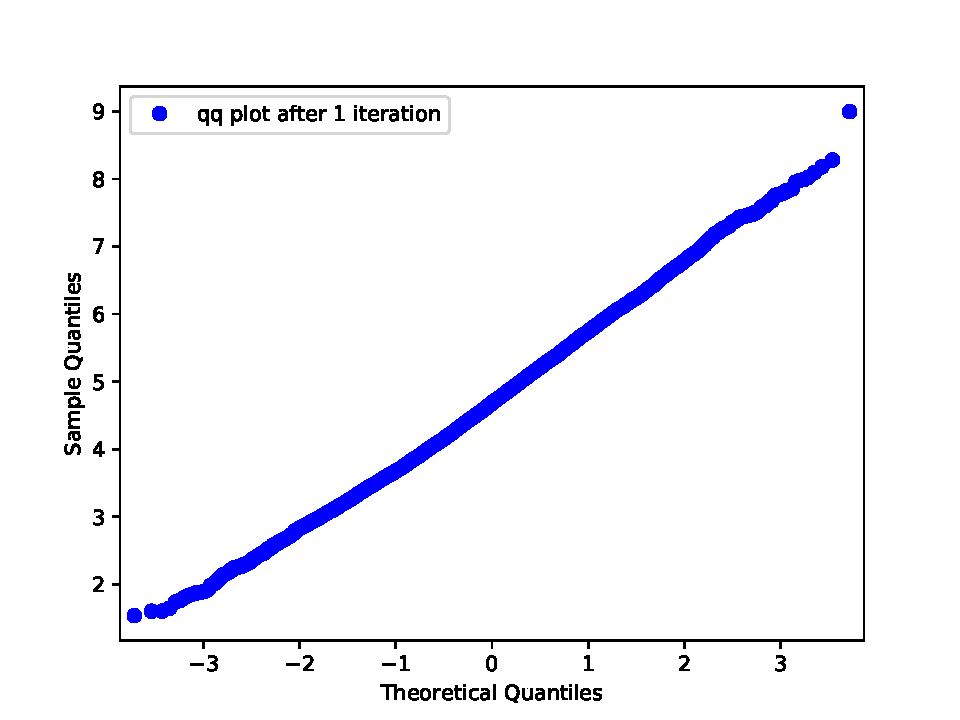
\includegraphics[width=0.4\textwidth]{../imgs/harmonic_oscillator_track/track_10010000_qq_1.pdf}
		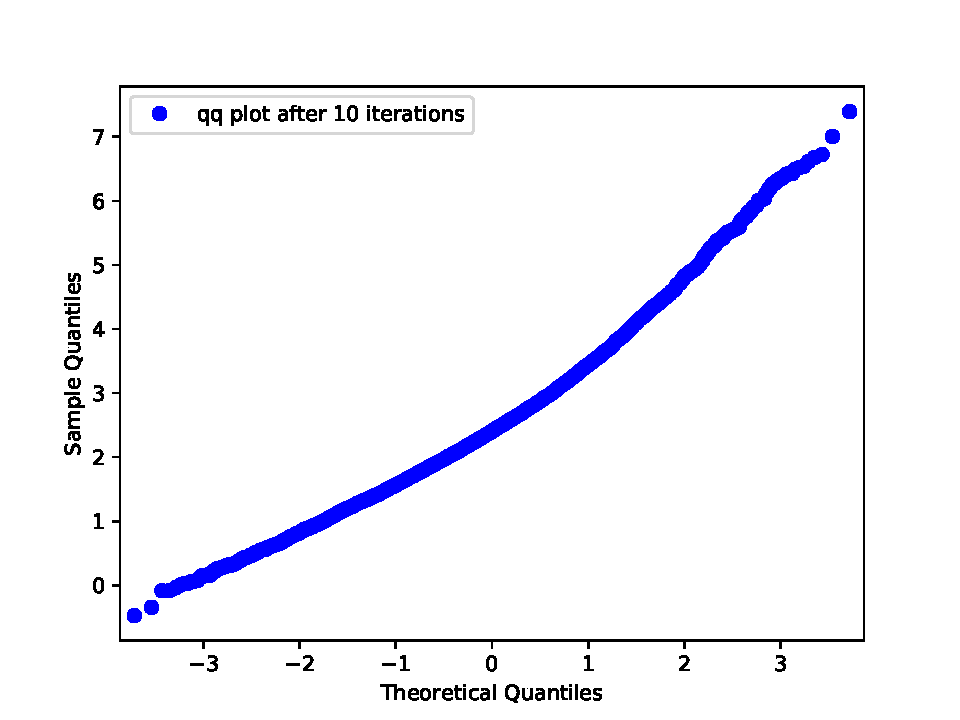
\includegraphics[width=0.4\textwidth]{../imgs/harmonic_oscillator_track/track_10010000_qq_10.pdf}
		\\
		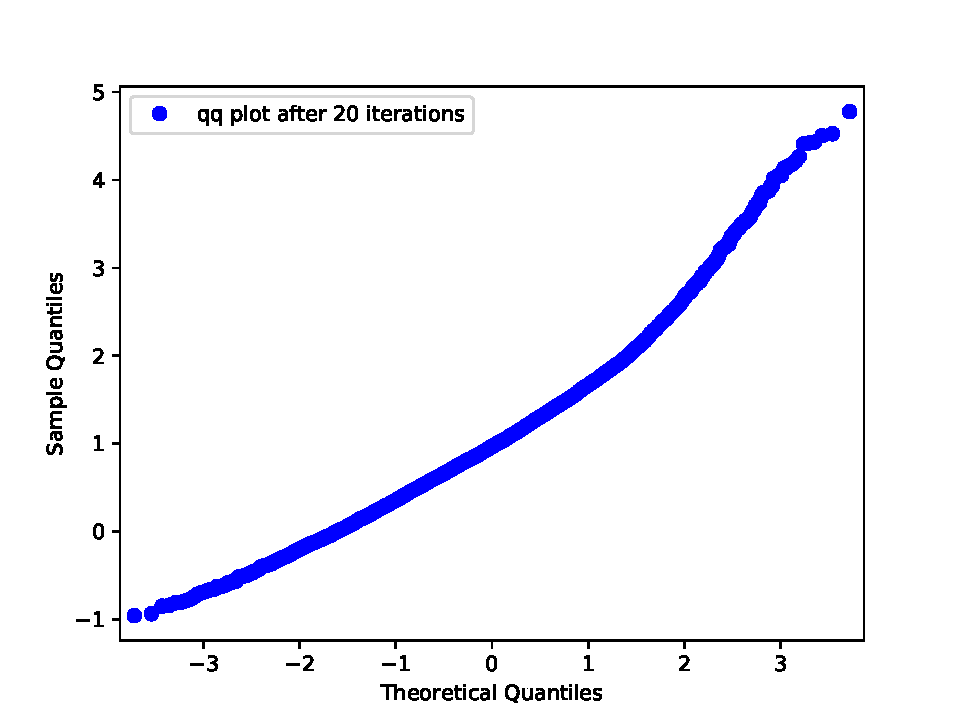
\includegraphics[width=0.4\textwidth]{../imgs/harmonic_oscillator_track/track_10010000_qq_20.pdf}
		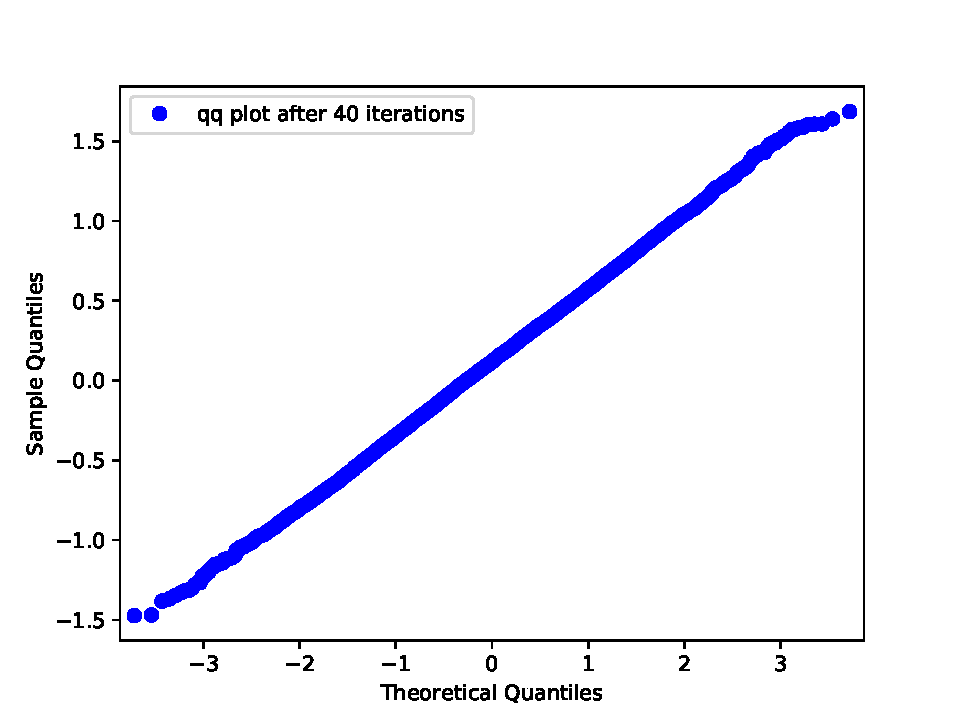
\includegraphics[width=0.4\textwidth]{../imgs/harmonic_oscillator_track/track_10010000_qq_40.pdf}
		\\
		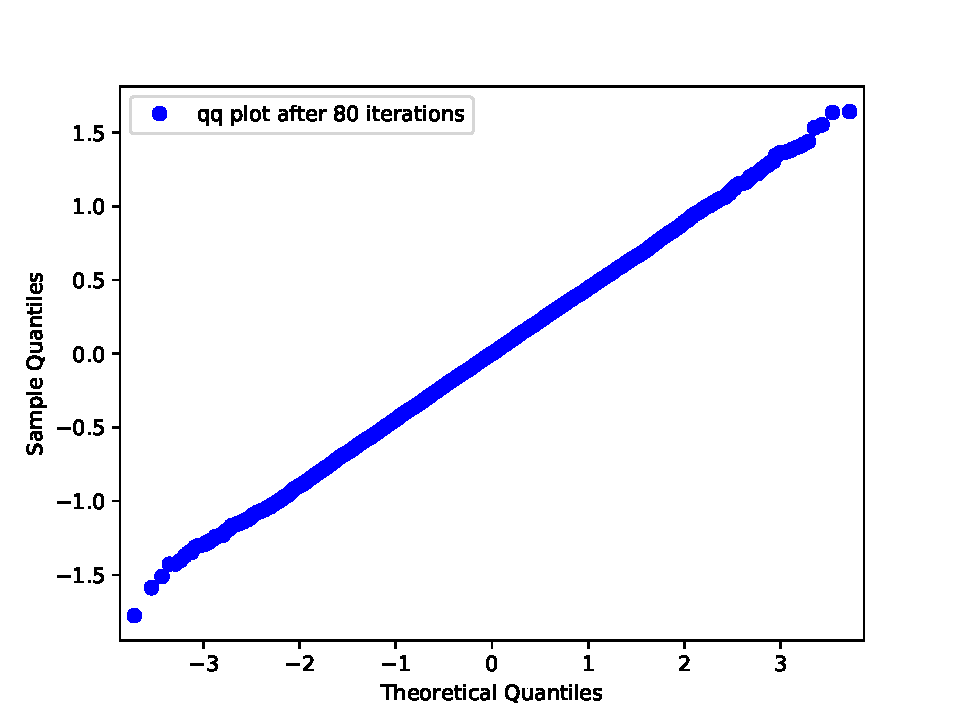
\includegraphics[width=0.4\textwidth]{../imgs/harmonic_oscillator_track/track_10010000_qq_80.pdf}
		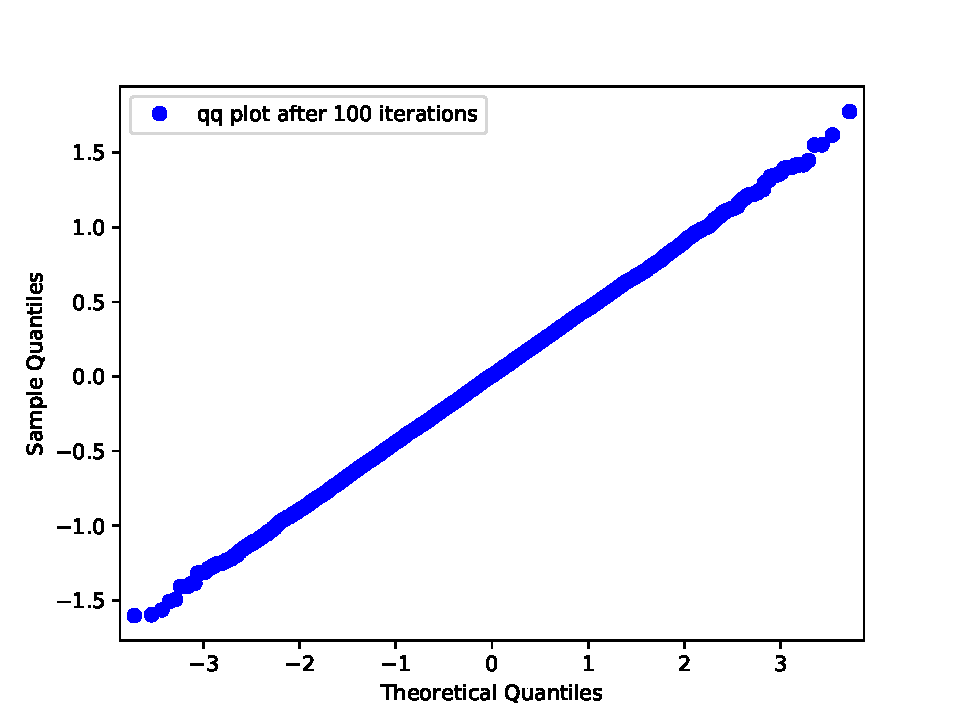
\includegraphics[width=0.4\textwidth]{../imgs/harmonic_oscillator_track/track_10010000_qq_100.pdf}
		\caption{}
	\end{figure}
	\section{Discussion}
	\section{Summary and Outlook}
\end{document}